\def\year{2018}
\relax
\documentclass[letterpaper]{article}
\usepackage{aaai18}
\usepackage{amsfonts}       % blackboard math symbols
\usepackage{nicefrac}       % compact symbols for 1/2, etc.
\usepackage{microtype}      % microtypography

\usepackage{hyperref}
\usepackage{url}
\usepackage[table]{xcolor}
\usepackage{bbm}
\usepackage{booktabs}
\usepackage[T1]{fontenc}
\usepackage{fix-cm}
\usepackage{array}
\usepackage{epsfig}
%\usepackage{mathabx}
\usepackage{dsfont}
\usepackage{multirow}


\usepackage{times}
\usepackage{helvet}
\usepackage{courier}
\usepackage{graphicx}
\usepackage{bm}
\usepackage{amsmath,amssymb} % define this before the line numbering.
\usepackage{color}
%\usepackage[width=122mm,left=12mm,paperwidth=146mm,height=193mm,top=12mm,paperheight=217mm]{geometry}
\usepackage{bbm}
\usepackage{epstopdf}
\usepackage{caption}
\usepackage{subcaption}
\usepackage{enumitem}
\usepackage{calc}
\usepackage{multirow}
\usepackage{xspace}
\usepackage{booktabs}
\usepackage{mathrsfs}
\usepackage{array}

\newcommand{\figref}[1]{Fig\onedot~\ref{#1}}
\newcommand{\equref}[1]{Eq\onedot~\eqref{#1}}
\newcommand{\secref}[1]{Sec\onedot~\ref{#1}}
\newcommand{\tabref}[1]{Tab\onedot~\ref{#1}}
\newcommand{\thmref}[1]{Theorem~\ref{#1}}
\newcommand{\prgref}[1]{Program~\ref{#1}}
\newcommand{\algref}[1]{Alg\onedot~\ref{#1}}
\newcommand{\clmref}[1]{Claim~\ref{#1}}
\newcommand{\lemref}[1]{Lemma~\ref{#1}}
\newcommand{\ptyref}[1]{Property\onedot~\ref{#1}}
\newcommand{\ve}[1]{{\mathbf #1}} % for displaying a vector or matrix
\newcommand{\hua}[1]{{\mathcal #1}}
\newcommand{\scr}[1]{{\mathcal #1}}
\newcommand{\by}[2]{\ensuremath{#1 \! \times \! #2}}


%\makeatletter
\DeclareRobustCommand\onedot{\futurelet\@let@token\@onedot}
\def\onedot{\ifx\@let@token.\else.\null\fi\xspace}
\def\eg{\emph{e.g.}} 
\def\Eg{\emph{E.g}\onedot}
\def\any{\forall}
\def\ie{\emph{i.e.}} 
\def\Ie{\emph{I.e}\onedot}
\def\cf{\emph{cf}\onedot} 
\def\Cf{\emph{Cf}\onedot}
\def\etc{\emph{etc}\onedot} 
\def\vs{\emph{vs}\onedot}
\def\wrt{w.r.t\onedot} 
\def\dof{d.o.f\onedot}
\def\etal{\emph{et al.}}

\frenchspacing
\setlength{\pdfpagewidth}{8.5in}
\setlength{\pdfpageheight}{11in}

\setcounter{secnumdepth}{2}  

\makeatletter
\newcommand{\thickhline}{%
    \noalign {\ifnum 0=`}\fi \hrule height 1pt
    \futurelet \reserved@a \@xhline
}
\newcolumntype{"}{@{\hskip\tabcolsep\vrule width 1pt\hskip\tabcolsep}}
\makeatother

\begin{document}
% The file aaai.sty is the style file for AAAI Press 
% proceedings, working notes, and technical reports.
\title{Unsupervised Learning of Geometry from Videos with Edge-aware Depth-Normal Consistency}
\author{Paper ID: 1138}

% \setlength{\abovedisplayskip}{4pt}
% \setlength{\belowdisplayskip}{3pt}
% \setlength{\abovedisplayshortskip}{2pt}
% \setlength{\belowdisplayshortskip}{2pt}
%\setlength{\bibitemsep}{.2\baselineskip plus .05\baselineskip minus .05\baselineskip}
\maketitle

\begin{abstract}
    Learning to recontruct 2.5D geometry from video in an unsupervised manner with deep convolutional network (DCN) \cite{zhou2017unsupervised} is acctracting significant attention in recent years, 
    due to that it can be widely applied to unlabeled videos online for applications such as augment relality etc.
    In this paper, to better recover the geometry inside an image, we propose to jointly estimate depth and normal in the unsupervised learning pipeline. Our estimated depth is guaranteed to be consistent with predicted normals in 3D space, yielding much more robust results for both depth and normals. 
    Specifically, we introduce two layers, i.e. a depth to normal layer and a normal to depth layer.
    The depth to normal layer takes estimated depth for each pixel as input, and compute normal directions with inner product. Then given the normal and depth, the normal to depth layer outputs a regularized depth through local planar smoothness.
    Finally, to train the network we apply the photometric loss, and further require gradient smoothness for both depth and normals predictions. 
    We conducted experiments on both outdoor (KITTI) and indoor (NYUv2) videos, and show that our algorithm vastly outperform the state-of-arts, reducing both depth and normal error over 20$\%$ relatively, which demonstrates the benefits from the normal representation.
\end{abstract}



\vspace{-1.0\baselineskip}
\section{Introduction}
\label{sec:intro}
\vspace{-0.3\baselineskip}

% depth normal is natural ability, without groud truth
Human beings are professional in recovering the 3D geometry of observed natural scenes at a very detailed level in real-time, even from a single image. 
More impressively, we leaned to achieve this ability only through visual perception of consecutive changing of outside world and ego-motion, \ie watching videos. 
Practically, being able to do reconstruction for unlabeled videos can be widely applied to large amount of real applications like augmented reality, robotics \etc

Therefore, letting computer manage dense 3D reconstruction ability by watching videos is a central problem of computer vision. 
One group of approaches is geometric based method depend on feature matching, \eg structure from motion (SFM) \cite{wu2011visualsfm} \etc, or color matching, \eg DTAM \cite{NewcombeLD11}, \etc  Since our world exists in 3D space and the images generated follows camera geometry, as long as the matching from corresponding frames are correct, we can exactly solve the 3D structure. 
However, theoretically, those methods does not explain why human can also do reconstruction from a single image by observing videos. In addition, they can easily fail once the feature matching is wrong, \eg when SIFT \cite{lowe2004distinctive}  feature meets a wall with white color. 
Thus, geometric based methods do not have the ability to discover new reconstruction cues from videos, and ignore the information inside monocular images.

\begin{figure}
\centering
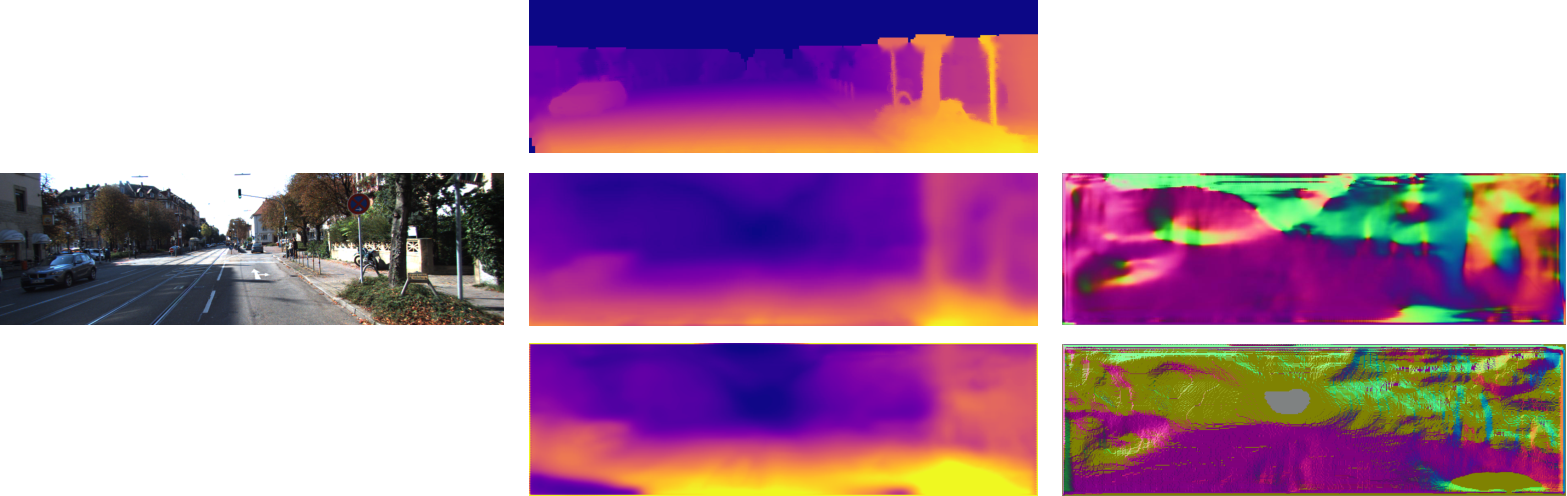
\includegraphics[width=0.45\textwidth]{figures/visual_comparison.pdf}
\caption{Comparison of visual outputs of our model with and without depth-normal consistency. Top to bottom: (b) ground truth depth and normal, (c) our results with depth-normal consistency, (d) our results without depth-normal consistency. Note in the red circle region, our model with depth-normal consistency predicts both depth and normal correct, but the model without depth-normal consistency fails in normal estimation.}
\label{fig:visual_comparison}
\vspace{-1.3\baselineskip}
\end{figure}

Another way to do 3D reconstruction is learning based method, where the reconstruction cues can be incrementally discovered and applied by keeping feeding in unobserved videos. Currently, with the development of pixel-wise prediction via deep learning such as fully convolutional network (FCN) \cite{long2015fully}, supervised learning of depth, \eg \cite{eigen2014depth,ummenhofer2016demon}, achieved impressive results over public datasets like KITTI \cite{}, NYUv2 \cite{silberman2012indoor} and SUN3D \cite{xiao2013sun3d}. 
Nevertheless, collecting ground truth depth is almost impossible for most online videos, where the learned models are hard to generalize. 
Thus, learning depth with unlabeled videos attracts lots of attention in recent years.
Garg \etal \cite{godard2016unsupervised} try to use FCN to predict depth from a single image, by using photometric matching from stereo pairs, and back-propagate the matching error to the network. Later works \cite{zhou2017unsupervised,Vijayanarasimhan17} extends to using information from consecutive video frames by introducing camera ego-motion. 
Although those methods are able to do single image depth estimation, the results are still far from satisfactory. As shown at \figref{fig:visual_comparison}(d), the depth results from \cite{zhou2017unsupervised} does not well represent the structure of scene, especially when visualized with computed normals. 
This is mostly due to photometric matching is ambiguous, \ie a color in source frames can be matched to multiple similar colors in target frames. Although researchers usually use smoothness of depth \cite{zhou2017unsupervised} to reduce the ambiguity, it is often a weak constraint over neighboring pixels, yielding non-satisfied normal results.

\begin{figure*}[t]
\centering
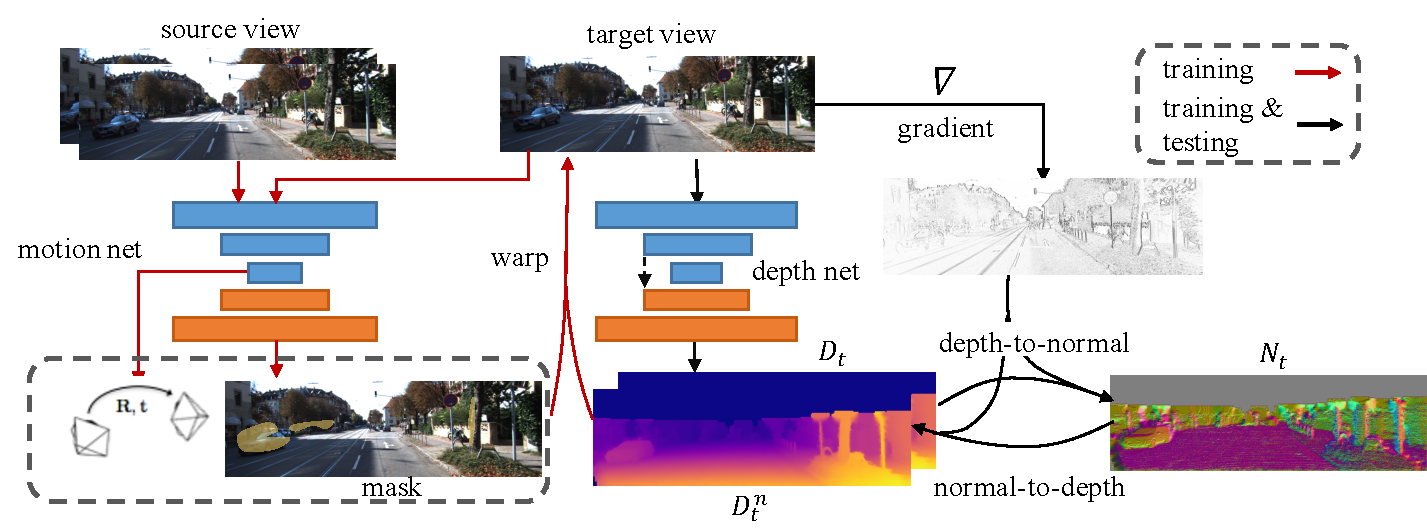
\includegraphics[width=0.85\textwidth]{figures/pipeline.pdf}
\caption{Framework of our approach (Details at \secref{sub:framework}).}
\label{fig:pipeline}
\vspace{-1.3\baselineskip}
\end{figure*}
Our work falls in the scope of learning based 3D reconstruction with videos following the work of \cite{zhou2017unsupervised}, but is a step further towards learning a regularized 3D geometry with particular awareness of normal representation. 
We are motivated by the fact that human beings are able to explicitly point out the normal direction of each pixel in an image. Actually, we are more sensitive to normal than depth, \eg one could precisely point out the normal direction of a pixel while could only roughly know the exact depth. 
Thus, we embed the normals representation inside the network as regularization layers, and enforce the prediction consistency with depth (\secref{sec:approach}).
There are several advantages of having normal estimated. For instance, it gives explicit understanding of normal for learned models.  In addition, it provides higher order interaction between estimated depths, which is beyond local neighbor relationships. Last, additional operations, \eg Manhattan assumption, over normals could be further integrated.
%Last but not the least, additional relationship, such as Manhattan world \cite{}, could be easily integrated with nor.
As shown at \figref{fig:visual_comparison}(c), with the help of normal, our recovered geometry is comparably better. We did extensive experiments over the publish KITTI and NYUv2 dataset for 3D reconstruction, and show our algorithm can achieve relative 20$\%$ improvement over the state-of-the-art method on depth estimation and 10$\%$ improvement on predicted normals. More importantly, the training converges much faster. These demonstrate the efficiency and effectiveness of our approach.
% recent work stereo, (eccv 2016, cvpr 2017), motion (cvpr 2017)
% matching can be easy, keep local structure for regularize depth is important,  

% normal is the most important structure that can explicit represent, no work on this

% we focus on 1: regularize depth, 2: explicit represent normal, 3: enforce the consistency


\vspace{-0.6\baselineskip}
\subsection{Framework}
\label{sub:framework}
\vspace{-0.3\baselineskip}

\figref{fig:pipeline} illustrate an overview of our approach. For training, we apply supervision from view synthesis following \cite{zhou2017unsupervised}. Specifically, the depth network (middle) takes only the target view as input, and
outputs a per-pixel depth map $D_t$, based on which a normal map $N_t$ is generated by the depth-to-normal layer. Then, given the $D_t$ and $N_t$, a new depth map $D_t^n$ is estimated from the normal-to-depth layer using local orthogonal compatibility between depth and normals. Both of the layers takes in image gradient to avoid non-compatible pixels involving in depth and normal conversion (detailed in \secref{sec:approach}).
Then, the new depth map $D_t^n$, combined with poses and mask predicted from the pose network (left), are then used to inversely warp the source views to reconstruct the target view, and errors are back propagated through both networks. Here the normal representation naturally serves as a regularization for depth estimation. Finally, for training loss, additional to the usually used photometric reconstruction loss, we also add in smoothness over normals, which induces higher order interaction between pixels (\secref{sub:training_losses})

After the model is trained, given a new image,  we first infer per-pixel depth value and then compute the normal value, yielding consistent prediction between the two predictions.
% problem normal can be locally estimated , while depth need global.  Another brach purely for normal


% In summary, the contributions of this paper lie in three folds:
% \begin{enumerate}
%     \item We provide to explicitly represent normal from images via unsupervised depth estimation, which is useful in real applications and serves as a regularization for depth prediction.
%     \item We

% \end{enumerate}



\vspace{-0.5\baselineskip}
\section{Related Work}
\label{sec:related}
\vspace{-0.3\baselineskip}

\textbf{~~~Structure from motion and single view geometry.}
As discussed in \secref{sec:intro}, geometry based methods, such as SFM~\cite{wu2011visualsfm}, ORB-SLAM~\cite{mur2015orb}, DTAM~\cite{NewcombeLD11}, rely on feature matching, which could be effective and efficient in many cases. 
However, they can fail at low texture, or drastic change of visual perspective \etc. More importantly, it can not extend to single view reconstruction where humans are good at.
Traditionally, specific rules are developed for single view geometry. Methods are dependent on either computing vanishing point~\cite{HoiemEH07}, following rules of BRDF~\cite{prados2006shape}, or abstract the scenes with major plane and box representations~\cite{DBLP:conf/iccv/SchwingFPU13,DBLP:conf/3dim/SrajerSPP14} \etc. Those methods can only obtain sparse geometry representations, and some of them require certain assumptions (\textit{e.g.} Lambertian, Manhattan world).

\textbf{Supervised single view geometry via CNN.}
With the advance of deep neural networks and their strong feature representation, dense geometry, i.e., pixel-wise depth and normal maps, can be readily estimated from a single image~\cite{wang2015designing,eigen2015predicting,laina2016deeper}. The learned CNN model show significant improvement comparing to other strategies based on hand-crafted features~\cite{karsch2014depth,ladicky2014pulling,zeisl2014discriminatively}. Others tried to improve the estimation further by appending a conditional random field (CRF)~\cite{DBLP:conf/cvpr/WangSLCPY15,Liu_2015_CVPR,li2015depth}. 
However, most works regard depth and normal predictions as independent tasks. \cite{peng2016depth} point out their correlations over large planar regions, and regularize the prediction using a dense CRF~\cite{kong2015intrinsic}, which improved the results on both depth and normal. However, all those methods require densely labeled ground truths, which are expensive to label in natural environments.

 % Long-range context and semantic cues are also incorporated in later works to refine the dense prediction by combining the networks with conditional random fields (CRF)~\cite{DBLP:conf/cvpr/WangSLCPY15, Liu_2015_CVPR, li2015depth, Wang_2015_CVPR}. Most recently, Eigen \textit{et al.}~\cite{DBLP:conf/iccv/EigenF15} further integrate depth and normal estimation into a large multi-scale network structure, which significantly improves the geometry estimation accuracy. Nevertheless, the output of the networks still lacks regularization over planar surfaces due to the adoption of pixel-wise loss functions during network training, resulting in unsatisfactory experience in 3D image editing applications.


%Later, the depth estimation from single-view input image is inherently an ill-posed problem which can only be solved with priors and semantic understanding of the scene - tasks that the convnets are good at. 
% There is a chain of works that propose learning depth/normal maps with deep convnets supervised with dense ground truth maps. \cite{liu2016learning} proposed to combine a convnet with a superpixel-based conditional random field (CRF) model, and to learn unary and pairwise terms for the depth map. Ladicky \etal \cite{ladicky2014pulling} incorporate semantics into their model to improve the per pixel depth estimation. Karsch \etal \cite{karsch2014depth} attempt to produce more consistent image level predictions by copying whole image depth from the training set, which requires the entire training set to be available during test time. Eigen \etal \cite{eigen2014depth,eigen2015predicting} showed it is possible to produce dense per pixel depth estimation through a two-scale deep network, trained on images and their corresponding ground truth depth maps. Many works have built upon this method using techniques like CRFs to improve accuracy \cite{li2015depth}, replacing regression loss with classification loss \cite{cao2017estimating}, implementing more robust loss function \cite{laina2016deeper}.

% Wang \etal \cite{wang2015designing} also built upon the basic idea of \cite{eigen2014depth} and incorporate scene geometrical priors to help learning, in the related problem of normal estimation. Data-driven normal estimation has not been long since the first approach, that directly tries to estimate surface normals from the data was proposed by Fouhey \etal \cite{fouhey2013data}.  Both this work and \cite{zeisl2014discriminatively} proposed by Ladicky \etal used hand-crafted features like texton, SIFT, local quantized ternary patterns. Li \etal \cite{\cite{li2015depth}} first proposed to estimate depth and normal jointly and showed performance gain. 

\textbf{Unsupervised single view geometry.}
Videos are easy to obtain at the present age, while hold much richer 3D information than single images. Thus, it attracts lots of interests if single view geometry can be learned through feature matching from videos. Recently, several deep learning methods have been proposed based on such an intuition. Deep3D \cite{xie2016deep3d} learns to generate the right view from the given left view by supervision of a stereo pair. In order to do back-propagation to depth values, it quantizes the depth space and trains to select the right one. 
% Video holds a great potential towards semantically meaningful visual representations. Recently, there have been a small number of deep network based methods for depth estimation. 
% DeepStereo \cite{flynn2016deepstereo} introduced a novel view synthesis network, while . This network generates new view images by selecting pixels from nearby images. The most appropriate depth values are selected to sample pixel values from neighboring images, based on plane sweep volume.
Concurrently, \cite{GargBR16} applied the similar supervision from stereo pairs, while the depth is kept continuous, They apply Taylor expansion to approximate the gradient for depth. \cite{godard2016unsupervised} extend Garg's work by including depth smoothness loss and left-right depth consistency. Most recently, \cite{zhou2017unsupervised} induces camera pose estimation into the training pipeline, which makes depth learning possible from monocular videos. However, they only focus on rigid scene without the ability to deal with moving objects. At the same time, \cite{kuznietsov2017semi} proposed a network to include modeling rigid object motion. Although vastly developed for depth estimation from video, normal information, which is also highly interesting for geometry prediction, has not been considered inside the pipeline. This paper fills in the missing part, and show that normal can serve as a natural regularization for depth estimation, which significantly improves the state-of-the-art performance. Finally, with our designed loss, we are able to  learn the indoor geometry where \cite{zhou2017unsupervised} usually fails to estimate.

% To deal with the problem of occlusion boundary caused by the rigid scene transformation and moving object, they proposed to mask out all these boundaries.

\section{Preliminaries}
\label{sec:preliminaries}
In order to make the paper self-contained, we first introduce several preliminaries proposed in the unsupervised learning pipelines \cite{zhou2017unsupervised,}. The core idea behind, as discussed in \ref{sec:related}, is inverse warping from target view to source view with awareness of 3D geometry, as illustrated in Fig. \ref{fig:3d_warping}(a), which we will elaborate in the following paragraphs.

\textbf{Perspective projection between multiple views.}
Let $D(x_t)$ be the depth value of the target view at image coordinate $x_t$, and $\ve{K}$ be the intrinsic parameter of the camera. Suppose the relative pose from the target view to source view is a rigid transformation $\ve{T}_{t\rightarrow s} = \{\ve{R} | \ve{t}\} \in \hua{S}\hua{E}(3)$, and $h(x)$ is the homogeneous coordinate given $x$. The perspective warping to localize corresponding pixels can be formulated as, 
\begin{align}
\label{eqn:warp}
D(x_s)h(x_s) = \ve{K}\ve{T}_{t\rightarrow s}D(x_t)\ve{K}^{-1}h(x_t),
\end{align}
and the image coordinate $x_s$ can be obtained by dehomogenisation of $d(x_s)h(x_s)$. Thus, $x_s$ and $x_t$ is a pair of matching coordinates, and we are able to compare the similarity between the two to valide the correctness of geometry.


\paragraph{Photometric error from view synthesis.} 
\label{chap:warping}
%that the color of each pixel is necessarily be similar after perspective projection for a static rigid scene
Given pixel matching pairs between target and source view, \ie $I_t$ and $I_s$, we can synthesis a target view from the given source view through bilinear interpolation~\cite{} $\hat{I_s}$ as illustrated in Fig. \ref{fig:3d_warping}(b). 
Then, under the assumption of Lambertian and a static rigid scene, average photometric error is often used to recover the depth map $D$ for the target view and the relative pose, \eg \cite{DBLP:conf/iccv/NewcombeLD11, zhou2017unsupervised}. 
However, as pointed out by Zhou \etal \cite{zhou2017unsupervised}, this assumption is not always true, due to the fact of existing moving object and occlusion. Thus, an explainability mask $\ve{M}$ is induced to leverage the issue. Formally, the masked photometric error is,

\begin{align}
\label{eqn:warp}
&\scr{E}_{vs}(D, \hua{T}, \hua{M}) = \sum_{s=1}^{N}\sum_{x_t}\ve{M}_s(x_t)|I_t(x_t) - \hat{I_s}(x_t)|, \\
&\text{s.t. ~~} d(x) > 0, \any \ve{M}_s(x)\in [0, 1],
\end{align}
where $\{I_s\}_{s=1}^{N}$ is the set of source views, and $\hua{T}$ is a set of transformation from target view to each of the source views. 
$\hua{M} = \{\ve{M}_s\}$ is a set of explainability masks, and $\ve{M}_s(x_t) \in [0, 1]$ is the weight to add error at $x_t$ from source view $s$.

%One main supervision of our framework comes from novel view synthesis: given an input view of a scene and camera motion, synthesize an image of the scene seen from a different view. 
% We can synthesize an image of the target view given the image of source view, camera motion from target view to source view and depth map of target view, using 3D inverse warping. The process of warping is shown in Figure \ref{fig:3d_warping}. 
\begin{figure}
\centering
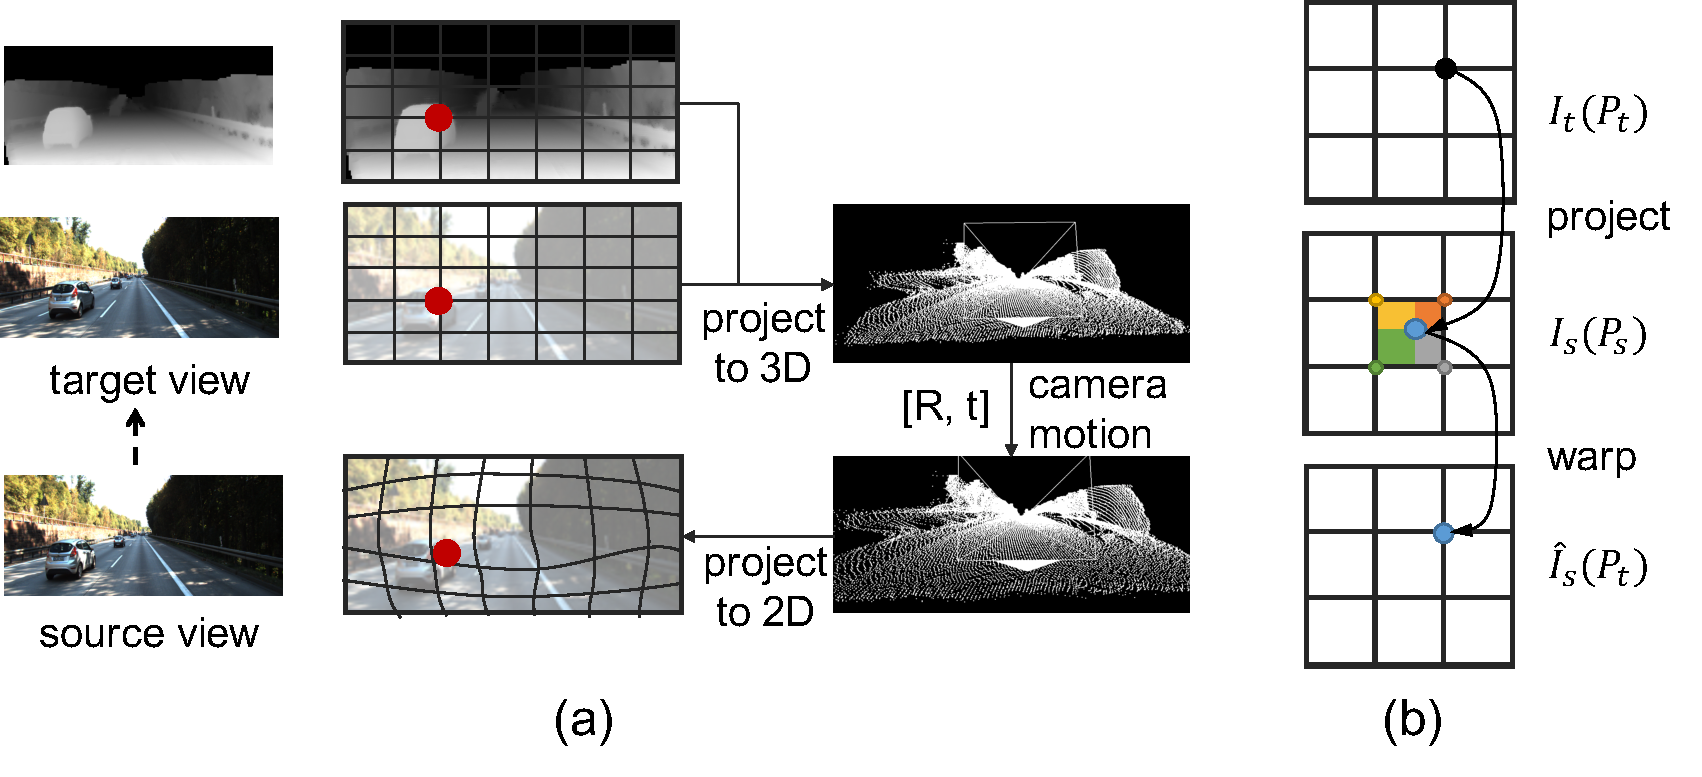
\includegraphics[width=0.5\textwidth]{figures/3d_warping.pdf}
\caption{Illustraion of (a) 3D inverse warping and (b) bilinear interpolation.}
\label{fig:3d_warping}
\end{figure}
% Each pixel (point on the grid) of depth map is first mapped onto 3D space. The 3D point cloud is transformed based on camera motion and then mapped back to 2D plane. Each grid point in target view corresponds to one point in source view. Similar to \cite{jaderberg2015spatial}, the bilinear interpolation is implemented to calculate each pixel value of warped image as a weighted sum of four nearest neighboring pixels in source image, weighted by the square area between the projected point and neighboring point, as shown in Figure \ref{fig:3d_warping} (b).

% The warping loss is a photometric difference between the target image and warped image. $$$$
% In which, $s$ iterates the number of source image, $p$ iterates each pixel in the image, $I_t$ is the target image, $I_s$ is the source image, $\hat{I_s} = \tau(I_s, D_t, Rt)$ is the warped image, $\tau$ is the warping function as introduced above.

\paragraph{Regularization.} 
As mentioned in Sec. \ref{sec:intro}, supervision based solely photometric error is ambiguous. One pixel could match to multiple candidates, especially at low-texture regions. In addition, there is trivial solution for explainability mask by setting all value to zero. Thus, to reduce depth ambiguity and encourage non-zero of masks, two regularization terms are applied, 
% One issue with using only view synthesis as supervision is that the back-propagation gradients are solely derived from the pixel value difference between one point in target image and weighted sum of its four neighboring points in source image. The warping loss will not be useful for learning where the point falls on low-texture regions. The predicted depth on these regions can be of any value as long as the warped region has the similar pixel value.  To overcome this issue, a prior knowledge of the scene geometry is incorporated for a smoothness loss:
\begin{align}
\label{eqn:regular}
\scr{E}_{s}(\ve{D}) &= \sum_{x_t}|\nabla^{2}_xD(x_t)|e^{-\alpha|\nabla_xI(x_t)|} + |\nabla^{2}_yD(x_t)|e^{-\alpha|\nabla_yI(x_t)|}& \\
\scr{E}_{m}(\hua{M}) &= -\sum_s\sum_{x_t}\log P(M_s(x_t) = 1) &
\end{align}
$\scr{E}_{s}(\ve{D})$ is a spatial smoothness term penalizes L1 norm of second-order gradients of depth along both x and y direction, encouraging depth value align in planar surface when no image gradient appears.
 % As depth discontinuity often happens at image gradients, the smoothness loss is weighted by the a function of image gradients to prevent smoothed depth at image gradients. 

Finally, multi-scale strategy is applied to the depth output, and the total loss for depth estimation from video is a joint functional from previous terms,
\begin{align}
\label{eqn:full}
\scr{E}_{f}(\{D_l\}, \hua{T}, \hua{M}) = \sum_l{\scr{E}_{vs}(\ve{D}_l,\hua{T},\hua{M}) + \lambda_s\scr{E}_{s}(\ve{D}_l) + \lambda_m\scr{E}_{m}(\hua{M}_l)}
\end{align}

Given the objective function, the photometric error can be back-propagated to depth, pose and mask networks by applying the spatial transform operation as proposed by~\cite{jaderberg2015spatial}, which supervises the learning process.


% \input{approach_new}
\vspace{-0\baselineskip}
\section{Geometry estimation with edge-aware depth-normal consistency}
\label{sec:approach}
\vspace{-0\baselineskip}

In our scenario, given a target image $I$, we aim at learning to estimate both depths and normals simultaneously. Formally, let $N$ be the predicted normals from our model, we embed it into the training pipeline and make it a regularization for depths estimation $D$, which helps to train a more robust model.

\vspace{-0\baselineskip}
\subsection{Framework}
\label{sub:framework}
\vspace{-0\baselineskip}

\figref{fig:pipeline} illustrates an overview of our approach. For training, we apply supervision from view synthesis following \cite{zhou2017unsupervised}. Specifically, the depth network (middle) takes only the target view as input, and
outputs a per-pixel depth map $D_t$, based on which a normal map $N_t$ is generated by the depth-to-normal layer. Then, given the $D_t$ and $N_t$, a new depth map $D_t^n$ is estimated from the normal-to-depth layer using local orthogonal compatibility between depth and normals. Both of the layers takes in image gradient to avoid non-compatible pixels involving in depth and normal conversion (detailed in \secref{sub:depth_and_normal_orthogonality}).
Then, the new depth map $D_t^n$, combined with poses and mask predicted from the motion network (left), are then used to inversely warp the source views to reconstruct the target view, and errors are back propagated through both networks. Here the normal representation naturally serves as a regularization for depth estimation. Finally, for training loss, additional to the usually used photometric reconstruction loss, we also add in smoothness over normals, which induces higher order interaction between pixels (\secref{sub:training_losses})

With the trained model, given a new image,  we infer per-pixel depth value and then compute the normal value, yielding consistent results between the two predictions.

\vspace{-0\baselineskip}
\subsection{Depth and normal orthogonality.}
\label{sub:depth_and_normal_orthogonality}
\vspace{-0\baselineskip}

In reconstruction, depth and normal are two strongly correlated information, which follows locally linear orthogonality. Formally, for each pixel $x_i$, such a correlation can be written as a quadratic minimization for a set of linear equations,
\begin{align}
\label{eq:orthognal}
&\scr{L}_{x_i}(D, N) = ||[\cdots,\omega_{ji}(\phi(x_j) - \phi(x_i)), \cdots]^T  N(x_i)||^2, \nonumber \\
&~\text{where~} \phi(x) = D(x)\ve{K}^{-1}h(x), \text{~} \|N(x_i)\|_2 = 1, \nonumber\\
&~\text{~~~~~~~~} \omega_{ji} > 0 \text{~~if~~} x_j \in \hua{N}(x_i)
\end{align}
where $\scr{N}(x_i)$ is a set of predefined neighborhood pixels of $x_i$, and $N(x_i)$ is a $3 \times 1$ vector. $\phi(x)$ is the back projected 3D point from 2D coordinate $x$. $\phi(x_j) - \phi(x_i)$ is a difference vector in 3D, and $\omega_{ji}$ is used to weight the equation for pixel $x_j$ \wrt $x_i$ which we will elaborate later.

As discussed in Sec. \ref{sec:related}, most previous works try to predict the two information independently without considering such a correlation, while only SURGE~\cite{peng2016depth} proposes to apply the consistency by a post CRF processing only over large planar regions. In our case, we enforce the consistency over the full image, and directly apply it to regularize the network to help the model learning. Specifically, to model their consistency, we developed two layers by solving \equref{eq:orthognal}, \ie a depth-to-normal layer and a normal-to-depth layer. 

\textbf{Infer normals from depths.} 
\label{chap:d2n}
Given a depth map $D$, for each point $x_i$, in order to get $N(x_i)$. From \equref{eq:orthognal}, we need to firstly define neighbors $\hua{N}(x_i)$ and weights $\omega_{ji}$, and then solve the set of linear equations. To deal with the first issue, we choose to use the 8-neighbor convention to compute normal directions, which considerably more robust than the 4-neighbor convention. 
However, it is not always good to equally weight all pixels due to depth discontinuity or dramatic normal changes may occur nearby. Thus, for computing $\omega_{ji}$, we weight more for neighboring pixels $x_j$ having similar color with $x_i$, while weight less otherwise. Formally, in our case, it is computed as $\omega_{ji} = \exp\{-\alpha|I(x_j) - I(x_i)|\}$ and $\alpha = 0.1$. 

For minimizing \equref{eq:orthognal}, one may apply a standard singular value decomposition (SVD) to obtain the solution. However, in our case, we need to embed such an operation in the network for training, and back-propagate the gradient respect to input depths. SVD is computationally non-efficient for back-propagation. Thus, we choose to use mean cross-product to approximate the minimization~\cite{jia2006using}, which is simpler and more efficient. 
Specifically, from the 8 neighbor pixels around $x_i = [m, n]$, we split them to 4 pairs, where each pair of pixels is perpendicular at 2D coordinate \wrt $x_i$, and in a counter clock-wise order, \ie $\hua{P}(x_i) = \{([m-1, n], [m, n+1]), \cdot, ([m+1, n-1], [m-1, n-1])\}$. 
Then, for each pair, cross product of their difference vector \wrt $x_i$ is computed, and the mean direction of the computed vectors is set as the normal direction of $x_i$. Formally, the solver for normals is written as, 
\begin{align}
\label{eq:cross}
&\ve{n} = \sum_{p\in\hua{P}}(\omega_{p_{0}, x_i}(\phi(p_{0}) - \phi(x_i)) \times \omega_{p_{1}, x_i}(\phi(p_{1}) - \phi(x_i))), \nonumber \\
&N(x_i) = \ve{n} / \|\ve{n}\|_2
\end{align}
The process of calculating the normal direction for $x_i$ using one pair of pixels is in Fig. \ref{fig:d2n}. 

%for each $q\in\theta(p)$, $R_q$ satisfies $(q-p)\cdot(r-p) = 0, \quad r \in R_q$.
% The normal direction of each point is computed based on the neighboring points after projecting to 3D space. The process of calculating normal direction of point $p$ is shown in Figure \ref{fig:d2n}. $\theta(p)$ is a set of neighboring (8) points of $p$. 
% Take point $q \in \theta(p)$ for example. $R_{q}$ is a set of points that satisfy the requirement: when projecting to 3D space, for $\hat{q} \in \hat{\theta}(p)$ and for $\hat{r} \in \hat{R}_{q}$, $(\hat(q)-\hat(p) \cdot (\hat{r} - \hat(p)) \neq 0)$. Symbols with hat represent corresponding points in 3D space. Theoretically, the cross-product of any two non-collinear (in 3D space) vectors connecting $\hat{p}$ and $\hat{\theta}(p)$ is the normal direction $N(p)$. To reduce the possiblity that the two vectors being collinear in 3D space, we require the vectors to be perpendicular when projected in 2D plane. The normal directions are averaged when iterating $q \in \theta(p)$, and then $l_2$ normalized to make it a unit vector. The normal direction is calculated as:

\begin{figure}
\centering
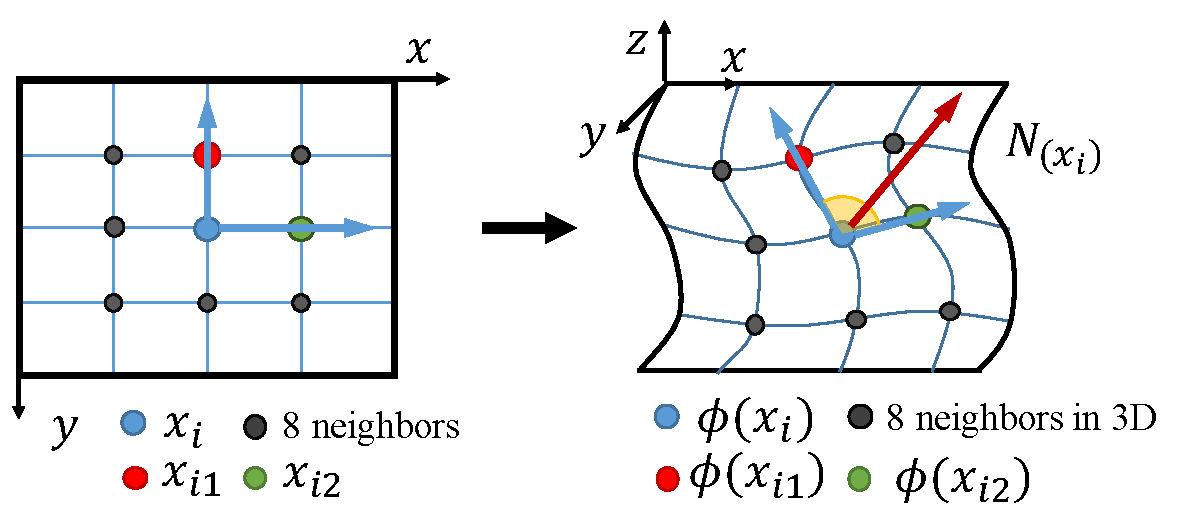
\includegraphics[width=0.5\textwidth]{figures/d2n.pdf}
\caption{Illustration of computing normal base on a pair of neighboring pixels. $x_i, x_{i1}, x_{i2}$ are 2D points, and 
$\phi(x_i), \phi(x_{i1}), \phi(x_{i2})$ are corresponding points projected to 3D space. 
The normal direction $N(x_i)$ is computed with cross product between $\phi(x_{i1}) - \phi(x_i)$ and $\phi(x_{i2}) - \phi(x_i)$.}
\vspace{-0.3\baselineskip}
\label{fig:d2n}
\end{figure}

\textbf{Compute depths from normals.} 
Due to the fact that we do not have ground truth normals for supervision, it is necessary to recover depths from normals to receive the supervision from photometric error as discussed in Sec.~\ref{sec:preliminaries}.
To recover depths, given normal map $N$, we still need to solve \equref{eq:orthognal}. However, there is no unique solution. Thus, to make it solvable, we provide an initial depth map $D_o$ as input, which might lack normal smoothness, \eg depth map from network output. Then, given $D_o(x_i)$, the depth solution for each neighboring pixel of $x_i$ is unique and can be easily computed. Formally, let $D_e(x_j | x_i) = \psi(D_o(x_i), N(x_i))$ be the solved depth value calculated for a neighbor pixel $x_j$ \wrt $x_i$. 
However, when computing over the full image, we still need to solve 8 equations jointly for each pixel of the 8 neighbors. Finally, by minimum square estimation (MSE), the solution for depth of $x_i$ is,
\begin{align}
\label{eq:depth}
D_n(x_j) = \sum_{i\in\hua{N}}\hat{\omega}_{ij}D_e(x_j | x_i), \text{~~}
\hat{\omega}_{ij} = \omega_{ij} / \sum_i{\omega_{ij}}
\end{align}

 %ormal2depth layer takes depth map and normal map as input and outputs a ``shifted" depth map. Take Figure \ref{fig:d2n} for example, the depth values of points $\theta(p)$ can be calcuated with the depth and normal direction of point $p$ known. From the calculation of normal direction, $(\hat{p} - \hat{q}) \cdot N(p) = 0$. When projecting points from 2D plane to 3D space, $\hat{p} = K^{-1}p$. $\hat{p} = (\hat{x}_p),\hat{y}_p,\hat{z}_p$, $p = (x_p, y_p, z_p)$ is a homogeneous 2D point and $z_p$ is the depth value of point $p$. $K^{-1}$ is the inverse of intrinsic matrix, which is determined by the camera. In linear the equation between depth and normal direction, $(K^{-1}(x_p, y_p, z_p) - K^{-1}(x_q, y_q, z_q))\cdot N(p) = 0, q\in\theta(p)$, the only unknown $z_q$, \ie  depth value of point $q$, has a unique solution. 

%As there are multiple points in the set $\theta(p)$, multiple depth maps can be recovered corresponding to each point $q \in \theta(p)$. In our pratice, the $\theta(p)$ includes 8 nearest points around point $p$. The 8 depth maps are weighted averaged to produce a reasonable depth output. As depth and normal discontinuity often happens where image gradients are large, similar to using image gradient in smoothness loss term, the image gradients are also calculated as weights to determine how much of each depth map contribute to final output. The output depth map is calculated as:
% $$z_p = \sum_{\theta(p)}z_q\frac{e^{(-\alpha|\partial_{\overrightarrow{p-q}}I_p|)}}{\sum_{\theta(p)}e^{(-\alpha|\partial_{\overrightarrow{p-q}}I_p|)}}, q\in\theta(p)$$
% In which, $\partial_{|\overrightarrow{p-q}}I_p|$ is the image gradient value along the $\overrightarrow{p-q}$ direction.
\vspace{-0\baselineskip}
\subsection{Training losses}
\label{sub:training_losses}
\vspace{-0.\baselineskip}

Given the consistency, in this section, we describe our training strategy. In order to supervise both the depth and normal predictions, we can directly apply the loss in \equref{eqn:full} by replacing the output from depth network $D_o$ with the output after our normal-to-depth layer $D_n$ to train the model. We show in our experiments (\secref{sec:experiments}), by doing this, we already outperform the previous state-of-the-art by around 10$\%$ in depth estimation using the same network architecture.

Additionally, with normal representation, we apply smoothness over neighboring normal values, which provides higher order interactive between pixels. Formally, the smoothness for normal has the same form as $\scr{L}_{s}$ in \equref{eqn:regular} for depth, while the first order gradient is applied, \ie $~\scr{L}_{s}(N, 1)$. 

Last but not the least, matching corresponding pixels between frames is another central factor to find correct geometry. Additional to the photometric error from matching pixel colors, matching image gradient is more robust to lighting variations, which was frequently applied in computing optical flow~\cite{li2017pyramidal}. 
In our case, we compute a gradient map of the target image and synthesized target images, and include the gradient matching error to our loss function. Formally, the loss is represented as,
\begin{equation}
\label{equ:gradient}
\scr{L}_{g}(D_n, \hua{T}, \hua{M}) = \sum_{s=1}^{S}\sum_{x_t}\ve{M}_s(x_t)\|\nabla I_t(x_t) - \nabla \hat{I_s}(x_t)\|_1, \nonumber
\end{equation}
%In the future, we hope to investigate more in matching criteria such as with stronger descriptors like SIFT~\cite{liu2011sift} or higher level convolutional features.

In summary, our final learning objective for multi-scale learning is,
\begin{align}
\label{eq:full_loss}
&\scr{L}(\hua{D}, \hua{N}, \hua{T}, \hua{M}) = \scr{L}_{o}(\{D_{nl}\}, \hua{T}, \hua{M}) + \nonumber\\
&\text{~~~~~~~~~}\sum_l\{\lambda_g\scr{L}_{g}(D_{nl},\hua{T},\hua{M}) + \lambda_n\scr{L}_{s}(N_l, 1)\}
\end{align}
where $\hua{D} = \{D_{nl}\}$ and $\hua{N} = \{N_{l}\}$ are the set of depth maps and normal maps for the target view.

%Our intuition is to train a CNN that is capable of modeling the geometry consistency of a mostly rigid scene. To facilitate the learning of the network, we explicitly propose to model the constraint between depth and normal. The training samples of the framework consist of frame sequences captured by a monocular moving camera.normalsize

\textbf{Model training.} For network architecture, similar to \cite{zhou2017unsupervised} and \cite{godard2016unsupervised}, we adopt the DispNet \cite{mayer2016large} architecture with skip connections as in \cite{zhou2017unsupervised}. All \textit{conv} layers are followed by a ReLU activation except for the top prediction layer. We train the network from scratch; since too many losses at beginning could be hard to optimize, we choose a two stage training strategy by first train the network with $\scr{L}_{o}$ with 5 epochs and then fine-tune it with the full loss for 1 epoch. We provide ablation study of each term in our experiments.


% To model a reasonable geometrical consistency, we propose the overall objective function as in Equation \ref{equ:1}.
% \begin{equation}
% \label{equ:1}
% \begin{split}
% L(D, I, Rt, \lambda) = L_{warp}(D, I, Rt) + L_{smooth}(D, N, I) \\
%  +  L_{grad}(D, I, Rt) + \lambda(L_{dn}(D, N))
% \end{split}
% \end{equation}
% Where

% This objective function is a Lagrange fuction aiming to minimize the loss term $L_{warp}(D, I, Rt) + L_{smooth}(D, N, I) \\
%  +  L_{grad}(D, I, Rt)$ subject to the constraint of geometrical constraint between depth map and normal map $L_dn(D, N) = 0$. The loss term consists of three components: photometric warping loss $L_{warp}(D, I, Rt)$, smoothness loss $L_{smooth}(D, N, I)$, image gradient matching loss $L_{grad}(D, I, Rt)$.

% By understanding the depth and normal 
 
% \subsection{Geometry consistency}

% As depth and surface normal are not independent under the same scene, 
% thus we model the 3D geometry consistency by explicitly incorporating the relationship of depth and normal into the training procedure and use the relationship as a regularization in the objective function. The regularization term $L_{dn}(D,N) = 0$ is realized by two layers in our framework: depth2normal layer and normal2depth layer.


% \subsection{Implementation details}

\vspace{-0\baselineskip}
\section{Experiments}
\label{sec:experiments}
\vspace{-0\baselineskip}

In this section, we introduce implementation details, datasets, evaluation metrics. An ablation study of how much each component of the framework contributes and a performance comparison with other supervised or unsupervised methods are also presented.

\vspace{-0\baselineskip}
\subsection{Implementation details.}
\vspace{-0\baselineskip}
Our framework is implemented with publicly available TensorfFlow \cite{abadi2016tensorflow} platform and has 34 million trainable variables in total. During training, Adam optimizer is applied with parameters $\beta_1 = 0.9$, $\beta_2=0.000$, $\epsilon=10^{-8}$. Learning rate and batch size are set to be $2\times10^{-3}$ and $4$ respectively. Batch normalization \cite{ioffe2015batch} is not used as we didn't observe a performance improvement with it. Following \cite{zhou2017unsupervised}, we use the same loss balancing for $\lambda_s, \lambda_m$, and correct the depth by a scale factor. We set $\lambda_n=1$ and $\lambda_g=\lambda_s$. %That is, multiplying the predicted depth by a factor $\hat{f}$: $\hat{f} = \mathrm{median}(D_{gt}) / \mathrm{median}(D_{pred})$. As the predicted depths are not absolute depth but defined up to a scale, 

The length of input sequence is fixed to be 3 and the input frames are resized to $128 \times 416$. The middle frame is treated as the target image and the other two are source images. Our network starts to show meaningful results after 3 epochs, and converges at the end of the 5th epoch. With a Nvidia Titan X (Pascal), the training process takes around 6 hours. The number of epochs and absolute time needed is much less than \cite{godard2016unsupervised} (50 epochs, 25 hours) and \cite{zhou2017unsupervised} (15 epochs).


\begin{table*}[t]
\centering
\caption{Depth performance of our framework variants on the KITTI split.}
\label{tbl:ablation}
\fontsize{8}{9}\selectfont
\bgroup
\def\arraystretch{1.2}
\begin{tabular}{c|c|c|c|c|c|c|c}
\thickhline
\multirow{2}{*}{Methods}  & \multicolumn{4}{c|}{Lower the better} & \multicolumn{3}{c}{Higher the better}                  \\ \cline{2-8} 
                          & Abs Rel  & Sq Rel  & RMSE  & RMSE log & $\delta < 1.25$ & $\delta < 1.25^2$ & $\delta < 1.25^3$ \\ \hline
Ours (no d-n)             & 0.208    & 2.286   & 7.462 & 0.297    & 0.693           & 0.875             & 0.948             \\
Ours (smooth no gradient) & 0.189    & 1.627   & 7.017 & 0.280    & 0.713           & 0.891             & 0.957             \\
Ours (no img grad for d-n)    & 0.179    & 1.566   & 7.247 & 0.272    & 0.720           & 0.895             & 0.959             \\
Ours (no normal smooth)   & 0.172    & 1.559   & 6.794 & 0.252    & 0.744           & 0.910             & 0.969             \\ \hline
\end{tabular}
\egroup
\vspace{-0\baselineskip}
\end{table*}

\vspace{-0.\baselineskip}
\subsection{Datasets and metrics}
\vspace{-0\baselineskip}
\textbf{~~~Training.}
Theorectically, our framework can be trained on any frame sequences captured with a monocular camera. To better compare with other methods, we evaluate on the popular KITTI 2015 \cite{geiger2012we} dataset. It is a large dataset suite for multiple tasks, including optical flow, 3D object detection, tracking, and road segmenations, \etc The raw data contains RGB and gray-scale videos, which are captured by stereo cameras from 61 scenes, with a typical image size of $1242 \times 375$.

In our experiments, videos captured by both left and right cameras are used for training, but treated independently. We follow the same training sequences as \cite{zhou2017unsupervised,eigen2014depth}, excluding frames from test scenes and static sequences. This results in 40,109 trainig sequences and 4431 validation sequences. Different from \cite{godard2016unsupervised}, no data augmentation has been performed.

\textbf{Testing.}
There are two sets of KITTI 2015 test data: (1) Eigen split contains 697 test images proposed by \cite{eigen2014depth}; (2) KITTI split contains 200 high-quality disparity images provided as part of official KITTI training set.  To better compare with other unsupervised and supervised methods, we present evaluations on both splits. 

The depth ground truth of Eigen split is generated by projecting 3D points scanned from Velodyne laser to the camera view. This produces depth values for less than 5\% of all pixels in the RGB images. To be consistent when comparing with other methods, the same crop as in \cite{eigen2014depth} is performed when testing. The depth ground truth of KITTI split contains sparse depth map with CAD models in place of moving cars. It provides better quality depth than projected Velodyne laser scanned points but has ambiguous depth value on object boundaries where the CAD model doesn't align with the images. The predicted depth is capped at 80 meters as in \cite{godard2016unsupervised} and \cite{zhou2017unsupervised}.

The normal ground truth for two splits is generated by applying our depth-to-normal layer on inpainted depth ground truth, where the same inpainting algorithm as \cite{silberman2012indoor} is used. For both depth and normal, following \cite{eigen2014depth}, only the pixels with laser ground truth are used.

\textbf{Metrics.} We apply the same depth evaluation and normal evaluation metrics as in \cite{eigen2015predicting}. For depth evaluation, we use the code provided by~\cite{zhou2017unsupervised} and for normal, we implement ourselves and verified the correctness through validating normal results of \cite{eigen2015predicting} over the NYUv2 dataset.

% Abs Rel: $\frac{1}{|D|}\sum_{d_{pred}\in D}|d_gt - d_{pred}|/d_gt$

% Sq Rel: $\frac{1}{|D|}\sum_{d_{pred}\in D}||d_gt - d_{pred}||^2/d_gt$

% RMSE: $\sqrt{\frac{1}{|D|}\sum_{d_{pred}\in D}||d_{gt} - d_{pred}||^2}$

% RMSE log: $\sqrt{\frac{1}{|D|}\sum_{d_{pred}\in D}||\log d_{gt} - \log d_{pred}||^2}$

% $\delta<thr$: $\%$ of $d_{pred}\in D$, s.t. $max(\frac{d_gt}{d_{pred}}, \frac{d_{pred}}{d_{gt}})<thr$

% mean: $\frac{1}{|N|}\sum_{n_{pred}\in N}(n_{gt}\cdot n_{pred})$

% median: $median([(n_{gt}\cdot n_{pred})]_{n_{pred} \in N})$

% degree: $\%$ of $n_{pred} \in N$, s.t. $(n_{gt}\cdot n_{pred}) < degree$


\vspace{-0\baselineskip}
\subsection{Ablation study}
\vspace{-0\baselineskip}
To investigate different components proposed in \secref{sec:approach}, we perform an ablation study by removing each one from our full model and evaluating on the KITTI split.

\textbf{Depth-normal consistency.} By removing normal-to-depth layer (\equref{eq:depth}), the inverse warping process (Sec. \ref{chap:warping}) takes an image and directly predicted depth map from the input. We show the performance at the row ``Ours (no d-n)" in Tab. \ref{tbl:ablation}. It is much worse than our full model on Kitti shown in Tab. \ref{tbl:sota}.
Notice that with depth-normal consistency, the network not only performs better but converges faster. In fact, our full model converges after 5 epochs, while the network without such consistency converges at 15th epoch.

% We explore the effectivness of adding image gradient into smoothness term.
\textbf{Image gradient in smoothness term.} To validate image gradient for depth and normal smoothness in \equref{eqn:regular}, 
we setting $\alpha=0$. The results is shown as ``Ours (smooth no gradient)" in Tab. \ref{tbl:ablation}. It makes less impoact than depth-normal consistency, but still helps the performance.

\textbf{Image gradient in normal-depth consistency.} We set $\omega=1$ in \equref{eq:orthognal}, thus there is no edge awareness in depth-normal consistency. As show at row ``Ours (no img grad for n-d)'', the results are again worse than our final results, which demonstrates the effectiveness by only enforcing the consistency between color similar pixels. % With image gradient in normal-to-depth layer, the normal direction will only contribute to those neighboring points $q$ where there is small image gradient between central point $p$ and $q$, \ie the two points most likely lie on the same plane. With such constraint, the depth evaluation performance is better. 
%We explore the impact of normal smoothness term by evaluating normal performance comparing framework 

\textbf{Normal smoothness.} Finally, by removing normal smoothness $\scr{L}_n$ in \equref{eq:full_loss}, we show the results at row ``Ours (no normal smooth)'' in Tab. \ref{tbl:ablation}, where it makes less impact for depth than other components, while still make reasonable contributions. However, it makes relatively more contributions for normal performance as shown in Tab. \ref{tbl:normal}.

%\textbf{Image gradient matching.} There is no obvious 

\vspace{-0\baselineskip}
\subsection{Comparison with other methods}
\vspace{-0\baselineskip}

To compare with other state-of-the-arts, we show performances on both KITTI and Eigen split. The depth evaluation results are shown in Tab. \ref{tbl:sota}. Our method outperforms some supervised methods \eg \cite{eigen2014depth}, \cite{liu2016learning} and unsupervised methods \cite{zhou2017unsupervised}, \cite{kuznietsov2017semi}, while slightly worse than \cite{godard2016unsupervised} and \cite{kuznietsov2017semi}. It is worth noting that \cite{kuznietsov2017semi} utilizes the depth ground truth and \cite{godard2016unsupervised} takes stereo image pairs as input, which implies the camera motion is known. On KITTI test split, our method outperforms \cite{godard2016unsupervised} on the ``Sq Rel'' metric. As ``Sq Rel'' penalizes large depth error, due to regularization, our results has much less outlier depths. Finally, we show some qualitative results in Fig. \ref{fig:examples}.

\begin{table*}[t]
\centering
\caption{Single view depth test results on Eigen split (upper part) and KITTI split(lower part). All methods in this table use KITTI dataset for traning and the test result is capped in the range 0-80 meters. Test result on KITTI test split of Zhou et al. 2017 is generated by using their released code to train on KITTI dataset only.}
\label{tbl:sota}
\fontsize{6.5}{7}\selectfont
\bgroup
\def\arraystretch{1.4}
\begin{tabular}{lllllllllll}
\thickhline
\multirow{2}{*}{Method}                                      & \multirow{2}{*}{Test data}                        & \multicolumn{2}{l}{Supervision} & \multicolumn{4}{l}{Lower the better} & \multicolumn{3}{l}{Higher the better}               \\ \cline{3-11} 
                                                             &                                                   & Depth          & Pose           & Abs Rel  & Sq Rel & RMSE  & RMSE log & $\delta < 1.25$ & $\delta<1.25^2$ & $\delta<1.25^3$ \\ \hline
\multicolumn{1}{l|}{Train set mean}                          & \multicolumn{1}{l|}{\multirow{8}{*}{Eigen split}} & \checkmark     &                & 0.403    & 5.530  & 8.709 & 0.403    & 0.593           & 0.776           & 0.878           \\
\multicolumn{1}{l|}{\cite{eigen2014depth} Coarse}            & \multicolumn{1}{l|}{}                             & \checkmark     &                & 0.214    & 1.605  & 6.563 & 0.292    & 0.673           & 0.884           & 0.957           \\
\multicolumn{1}{l|}{\cite{eigen2014depth} Fine}               & \multicolumn{1}{l|}{}                             & \checkmark     &                & 0.203    & 1.548  & 6.307 & 0.282    & 0.702           & 0.890           & 0.958           \\
\multicolumn{1}{l|}{\cite{kuznietsov2017semi} supervised}   & \multicolumn{1}{l|}{}                             & \checkmark     &                & 0.122    & 0.763  & 4.815 & 0.194    & 0.845           & 0.957           & 0.987           \\
\multicolumn{1}{l|}{\cite{kuznietsov2017semi} unsupervised} & \multicolumn{1}{l|}{}                             &                & \checkmark     & 0.308    & 9.367  & 8.700 & 0.367    & 0.752           & 0.904           & 0.952           \\
\multicolumn{1}{l|}{\cite{godard2016unsupervised}}                  & \multicolumn{1}{l|}{}                             &                & \checkmark     & 0.148    & 1.344  & 5.927 & 0.247    & 0.803           & 0.922           & 0.964           \\
\multicolumn{1}{l|}{\cite{zhou2017unsupervised}}                    & \multicolumn{1}{l|}{}                             &                &                & 0.208    & 1.768  & 6.856 & 0.283    & 0.678           & 0.885           & 0.957           \\
\multicolumn{1}{l|}{Ours}                                    & \multicolumn{1}{l|}{}                             &                &                & 0.182    & 1.481  & 6.501 & 0.267    & 0.725           & 0.906           & 0.963           \\ \hline
\multicolumn{1}{l|}{Train set mean}                          & \multicolumn{1}{r|}{\multirow{2}{*}{}}            & \checkmark     &                & 0.398    & 5.519  & 8.632 & 0.405    & 0.587           & 0.764           & 0.880           \\
\multicolumn{1}{l|}{\cite{godard2016unsupervised}}                  & \multicolumn{1}{r|}{}                             &                & \checkmark     & 0.124    & 1.388  & 6.125 & 0.217    & 0.841           & 0.936           & 0.975           \\
\multicolumn{1}{l|}{\cite{Vijayanarasimhan17}}        & \multicolumn{1}{l|}{KITTI split}                  &                &                & -        & -      & -     & 0.340    & -               & -               & -               \\
\multicolumn{1}{l|}{\cite{zhou2017unsupervised}}                    & \multicolumn{1}{l|}{\multirow{2}{*}{}}            &                &                & 0.216    & 2.255  & 7.422 & 0.299    & 0.686           & 0.873           & 0.951           \\
\multicolumn{1}{l|}{Ours}                                    & \multicolumn{1}{l|}{}                             &                &                & 0.1648   & 1.360  & 6.641 & 0.248    & 0.750           & 0.914           & 0.969           \\ \hline
\end{tabular}
\egroup
\vspace{-0.3\baselineskip}
\end{table*}


\begin{figure*}
\vspace{-0\baselineskip}
\centering
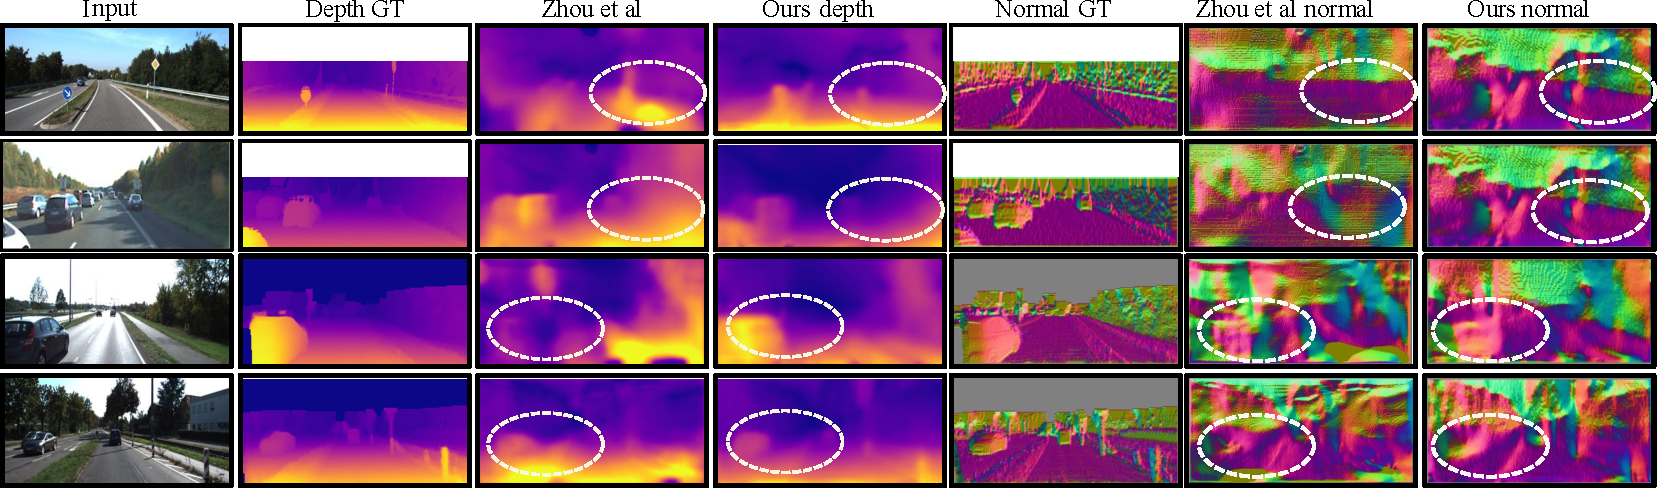
\includegraphics[width=\textwidth]{figures/examples_7col_comp-v2.pdf}
% \caption{Visual comparison of depth and normal results between \protect\cite{zhou2017unsupervised} and ours. As the original depth ground truth map comes from sparse laser measurement, the interpolated depth map is shown for better visualization. As can be seen from the depth estimation, our results preserve the small/thin structures which have similar color to other foregrounds (green circles). From the normal comparison, our results predict the road normal direction better and have no artifact. The edges in normal map are also preserved better in our results (yello circles).}
\caption{Visual comparison between \protect\cite{zhou2017unsupervised} and ours. We use the interpolated ground truth depths and reshape the image for better visualization. For both depths and normals, our results have less artifacts, reflect the scene layouts much better (as circled in the 1st and 2nd row) and preserve more detailed structures such as cars (as circled in the 3rd and 4th row). }
\vspace{-0\baselineskip}
\label{fig:examples}
\end{figure*}

\begin{figure}[h]
\centering
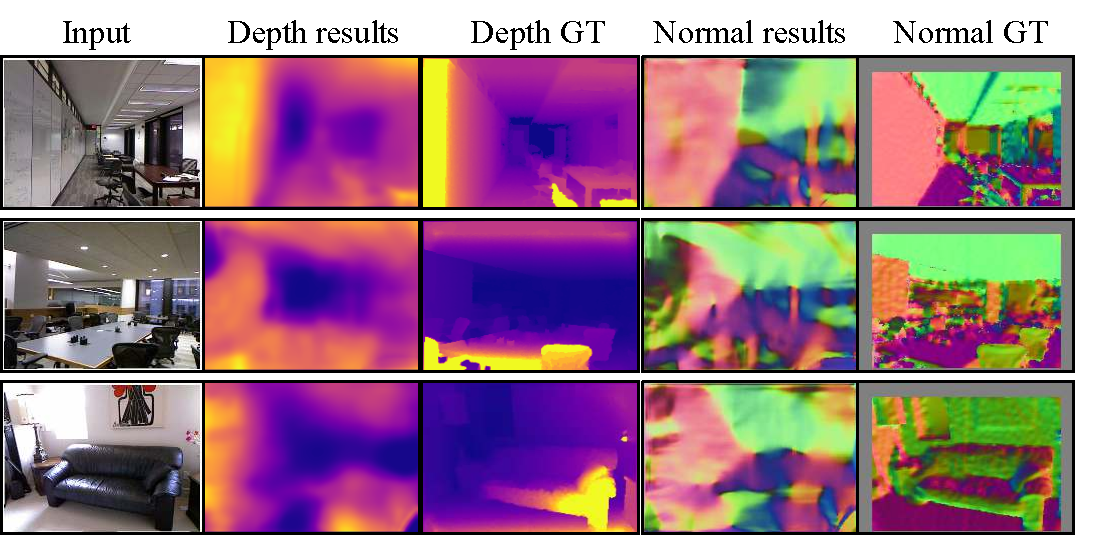
\includegraphics[width=0.5\textwidth]{figures/indoor_visual_comp.pdf}
\caption{Qualitative results of our framework on a subset of NYU v2 dataset.}
\vspace{-1.\baselineskip}
\label{fig:nyu_visual}
\end{figure}

To the best of our knowledge, there is no work reporting normal performance on the KITTI dataset. We thus compare the our normal predictions with that computed from the depth maps predicted by \cite{zhou2017unsupervised}. As shown in Tab. \ref{tbl:normal}, our method outperforms the baseline under all metrics. Additionally, to ensure the model is learned reasonably, we set up two naive baselines. ``Ground truth normal mean'' is that we set a mean normal direction for all pixels using ground truth normals. ``Pre-defined scene'' is that we separate the image to 4 parts using 4 lines connecting each image corder and image center. We set the bottom part having up-directed normal, left part having right-directed normal, right part having left-directed normal and top part with outward normals. Both of the baselines are significantly worse than our predicted model, demonstrating the correctness of the learned model.

%  and \cite{godard2016unsupervised}

% To our knowledge, there has not been works that report normal performance on KITTI 2015 dataset. We thus compare our normal performance with baseline methods and normals generated by applying depth-to-normal layer on depth maps of \cite{zhou2017unsupervised}. The baseline methods include ground truth normal mean, normals from pre-defined scene, our framework without second stage training, \ie without normal smoothness term and our full framework. As shown in Tab. \ref{tbl:normal}, our full model outperforms other methods under all metrics.

\begin{table}[t] \small
\centering
\caption{Normal performances of our method and some baseline methods.}
\label{tbl:normal}
\fontsize{6.5}{7}\selectfont
\bgroup
\def\arraystretch{1.2}
\begin{tabular}{l|c|c|c|c|c}
\thickhline
Method                        & Mean  & Median & $11.25^{\circ}$ & $22.5^{\circ}$  & $30^{\circ}$    \\ \hline
Ground truth normal mean      & 72.39 & 64.72  & 0.031 & 0.134 & 0.243 \\
Pre-defined scene             & 63.52 & 58.93  & 0.067 & 0.196 & 0.302 \\
\cite{zhou2017unsupervised} & 50.47 & 39.16  & 0.125 & 0.303 & 0.425 \\
Ours w/o normal smoothness    & 49.30 & 36.83  & 0.138 & 0.343 & 0.436 \\
Ours                          & 47.52 & 33.98  & 0.149 & 0.369 & 0.473 \\ \hline
\end{tabular}
\egroup
\vspace{-1.0\baselineskip}
\end{table}


\vspace{-0.8\baselineskip}
\paragraph{Indoor scene exploration.}
Besides the outdoor dataset, we also try to apply our framework on the indoor NYUv2 dataset \cite{silberman2012indoor}. We use a subset for some preliminary experiments. Specifically, ``study room" is picked and split for training and testing. We first try with our baseline method~\cite{zhou2017unsupervised}, and it fails to predict any reasonable depth maps. However, as shown in Fig. \ref{fig:nyu_visual}, our framework performs reasonably good on scenes that have multiple intersecting planes. Nevertheless, we still fail on scenes that have only a clutter of object. In the future, we plan to explore more on stronger feature matching rather than just using color matching, which may facilitate the learning under cluttered scenes.


\section{Conclusion} 
In this paper, we propose an unsupervised learning framework for joint depth and normal estimation via edge-aware depth and normal consistency. Our novel depth-normal regularization enforces the geoemetry consistency between different projections of the 3D scene, improving evaluation performances and also the training speed.
We present ablation experiments exploring each component of our framework and also on different scenes of images. Our results are comparable to some supervised methods, and achieve state-of-the-art performance among unsupervised monocular methods.

\paragraph{Future work.}
In future work, we will not be limited to unsupervised learning, while being able to stick in supervised training of joint normal and depth prediction for cross supervision, \eg using normal ground truth to regularize estimated depth.



% \newpage
\small
\bibliographystyle{aaai}
\bibliography{reference}

\end{document}
